\clearpage
\section{生成图检查与确认保存方案}
\label{sec:design-png}
模型生成的图先进入检查，通过展示检查后才进入预览。用户确认后才能将预览图保存为正式立绘。

\begin{figure}[H]
\centering
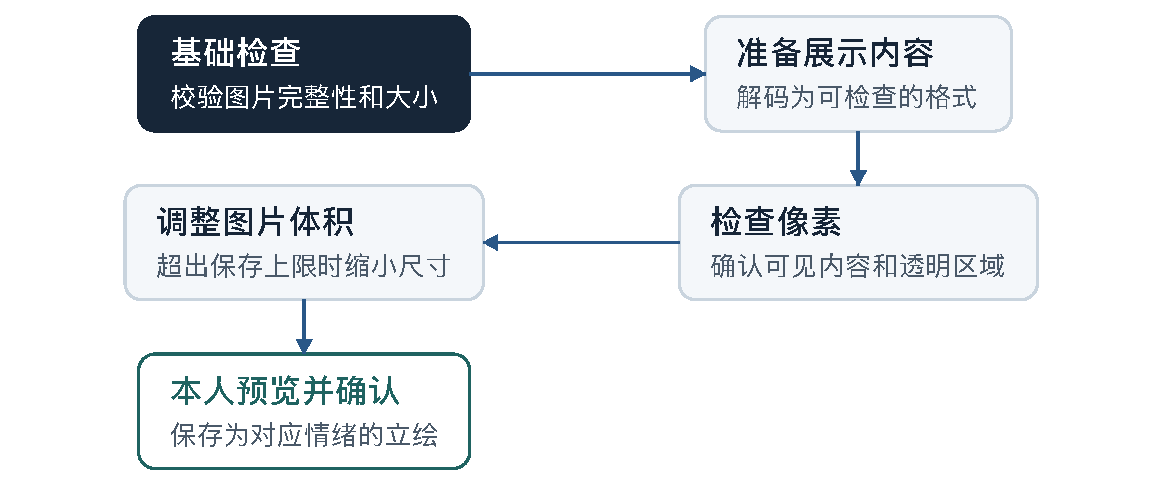
\includegraphics[width=\linewidth]{assets/design/png-save.pdf}
\caption{生成图检查、预览与确认保存流程}\label{fig:design-png-flow}
\end{figure}

服务端先校验 PNG 文件签名、数据块校验值、尺寸与解压长度，再将图片解码为 RGBA。图片须含可见像素，且至少 1\% 的像素透明度通道值小于 255。检查失败时结束任务并提示重新生成。

重编码后若超出 2\,000\,000 字节，逐步缩小尺寸，最终用同一份图片预览和保存。确认时，服务端核对任务归属、默认立绘的内容摘要及目标情绪图的版本。若素材不一致，保留预览并提示放弃后重新生成。

通过检查后，情绪图、任务完成状态和预览处理结果一起保存。比如确认开心立绘后，该图会成为开心状态的展示素材，任务也会标为已保存。

